\documentclass[a4paper, 12pt]{article}
\usepackage[utf8]{inputenc}
\usepackage[russian,english]{babel}
\usepackage[T2A]{fontenc}
\usepackage[left=10mm, top=20mm, right=10mm, bottom=15mm, footskip=13mm]{geometry}
\usepackage{indentfirst}
\usepackage{amsmath,amssymb}
\usepackage{graphicx}
\usepackage[italicdiff]{physics}
\usepackage{float}
\usepackage{array}
\usepackage{physics}
\graphicspath{ {shema/} {graphic/} }
\usepackage{caption}
\captionsetup[figure]{name=Рисунок}
  
\title{Отчет по лабораторной работе 1.3.1

Определение модуля Юнга на основе исследования деформаций растяжения и изгиба}

\author{Максим Осипов, Б03-504}
\date{01.10.2025}

\begin{document}
\maketitle
\newpage
\section{Аннотация}
В данной лабораторной работе экспериментально исследуется зависимость между напряжением и деформацией для упругих тел с целью определения модуля Юнга. Работа состоит из двух частей. В первой части изучается деформация одноосного растяжения проволоки с использованием прибора Лермантова, где удлинение измеряется по углу поворота зеркальца. Во второй части исследуется деформация чистого изгиба балки, опирающейся на две призмы. Модуль Юнга определяется по величине прогиба её середины под действием известной нагрузки, приложенной в центре. Для расчёта используются измеренные геометрические параметры стержня и расстояние между опорами.

\section{Теоретическая справка}
\subsection{Определение модуля Юнга по измерениям растяжения проволоки}


Для определения модуля Юнга по измерениям растяжения используется прибор Лермантова. Верхний конец проволоки прикреплен к консоли, а нижний - к цилиндру шарнирного кронштейна. На этот цилиндр опирается рычаг, связанный с зеркальцем, что позволяет измерять удлинение проволоки по углу поворота зеркальца.

\begin{figure}[h]
\centering
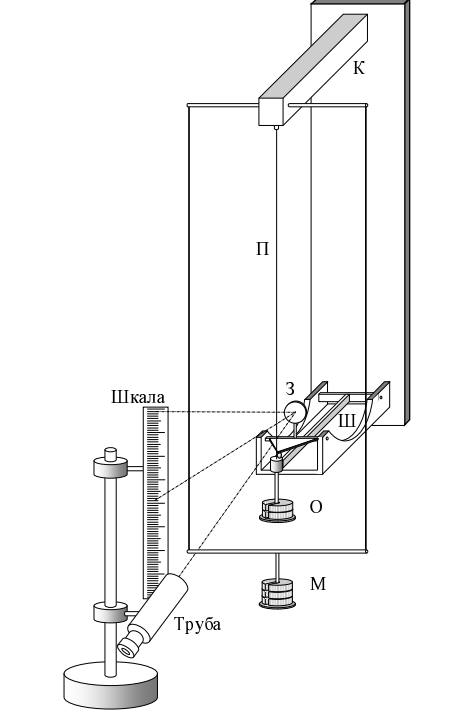
\includegraphics[width=0.4\linewidth]{прибор Лермантова.png}
\caption{Прибор Лермантова }
\label{fig:voltage_current}
\end{figure}

\newpage

\subsection{Определение модуля Юнга по измерениям изгиба}
Для определения модуля Юнга по измерениям изгиба используется установка, состоящая из прочной стойки с опорными призмами A и B. На ребра призм опирается исследуемый стержень. В середине стержня на призме подвешена площадка с грузами. Стрелу прогиба измеряют с помощью индикатора.

\begin{figure}[h]
\centering
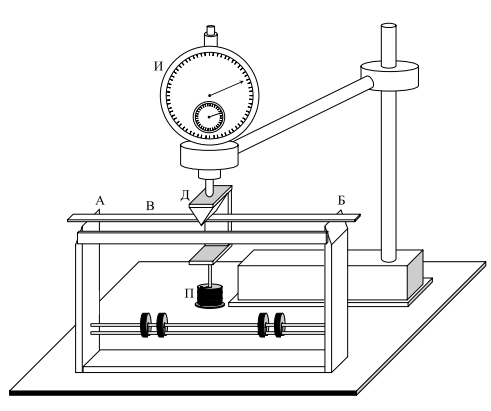
\includegraphics[width=0.5\linewidth]{схема установки.png}
\caption{Схема установки}
\label{fig:voltage_current}
\end{figure}

Модуль Юнга E материала стержня связан со стрелой прогиба y_max соотношением:

\[ E = \frac{P l^3}{4ab^3 y_{\max}} \]
где P - нагрузка, вызывающая прогиб стержня, l - расстояние между призмами A и B, a и b - ширина и высота сечения стержня.

\newpage
\section{Ход работы}

\subsection{Определение модуля Юнга по измерениям изгиба}

1. l_{AB} = l = 50\ \text{см}

2. Параметры балок

\begin{table}[h]
\centering
\caption{Параметры балок, погрешность 0.01 см}
\begin{tabular}{|c|c|c|c|c|c|}
\hline
Ш1 (дерево), см & Т1, см & Ш2 (металл), см & Т2, см & Ш3 (дерево2), см & Т3, см\\
\hline
2.05 & 1.05 & 2.14 & 0.40 & 2.02 & 1.07 \\
\hline
2.09 & 1.09 & 2.16 & 0.47 & 2.01 & 1.03 \\
\hline
2.05 & 1.09 & 2.15 & 0.46 & 2.06 & 1.06 \\
\hline
2.02 & 1.06 & 2.16 & 0.46 & 2.01 & 1.08 \\
\hline
2.04 & 1.05 & 2.16 & 0.48 & 2.04 & 1.04 \\
\hline
2.08 & 1.07 & 2.13 & 0.45 & 2.03 & 1.06 \\
\hline
2.05 & 1.07 & 2.15 & 0.47 & 2.04 & 1.07 \\
\hline
2.08 & 1.09 & 2.14 & 0.48 & 2.05 & 1.04 \\
\hline
2.05 & 1.06 & 2.15 & 0.45 & 2.04 & 1.05 \\
\hline
\multicolumn{6}{|c|}{Средние значения} \\
\hline
2.06 & 1.07 & 2.15 & 0.46 & 2.03 & 1.06 \\
\hline
\end{tabular}
\end{table}

3.Зависимость прогиба от нагрузки


\begin{table}[h]
\centering
\begin{minipage}{0.45\textwidth}
\centering
\caption{Зависимость прогиба от нагрузки (возрастание нагрузки)}
\begin{tabular}{|c|c|}
\hline
Нагрузка, H & прогиб, мм \\
\hline
0.0 & 0.0 \\
\hline
4.526 & 0.58 \\
\hline
9.458 & 1.25 \\
\hline
14.144 & 1.93 \\
\hline
18.873 & 2.61 \\
\hline
23.817 & 3.27 \\
\hline
28.73 & 4.02 \\
\hline
33.737 & 4.52 \\
\hline
\end{tabular}
\end{minipage}
\hfill
\begin{minipage}{0.45\textwidth}
\centering
\caption{Зависимость прогиба от нагрузки (убывание нагрузки)}
\begin{tabular}{|c|c|}
\hline
Нагрузка, H & прогиб, мм \\
\hline
33.737 & 4.52 \\
\hline
28.73 & 4.01 \\
\hline
23.817 & 3.3 \\
\hline
18.873 & 2.66 \\
\hline
14.144 & 1.97 \\
\hline
9.458 & 1.37 \\
\hline
4.526 & 0.68 \\
\hline
0.0 & 0.0 \\
\hline
\end{tabular}
\end{minipage}
\end{table}

Наблюдение: Балка вернулась в исходное положение


\begin{figure}[h]
\centering
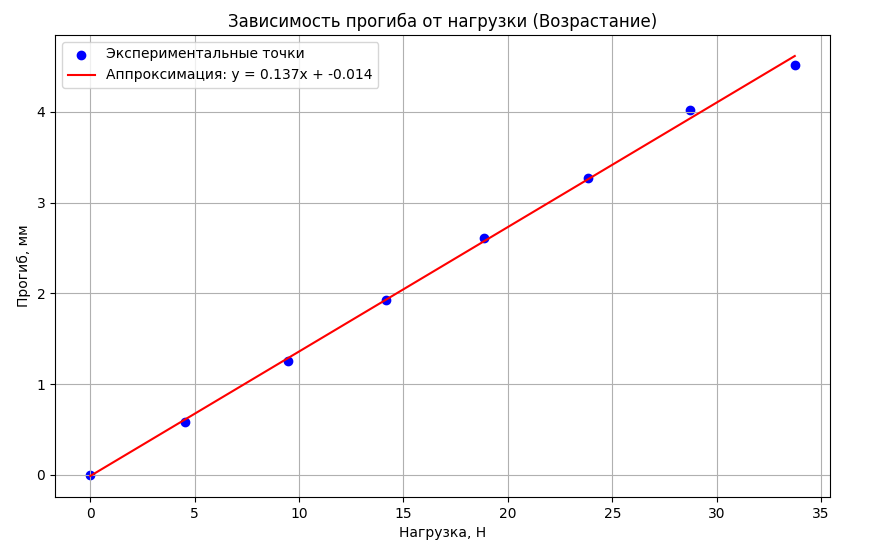
\includegraphics[width=0.8\linewidth]{Graph 1.png}
\caption{Коэффициент угла наклона (возрастание): 0.137; Модуль Юнга E = 19.04ГПа}
\label{fig:increase}
\end{figure}


\vspace{2cm} % Добавляем вертикальное пространство между картинками

\begin{figure}[h]
\centering
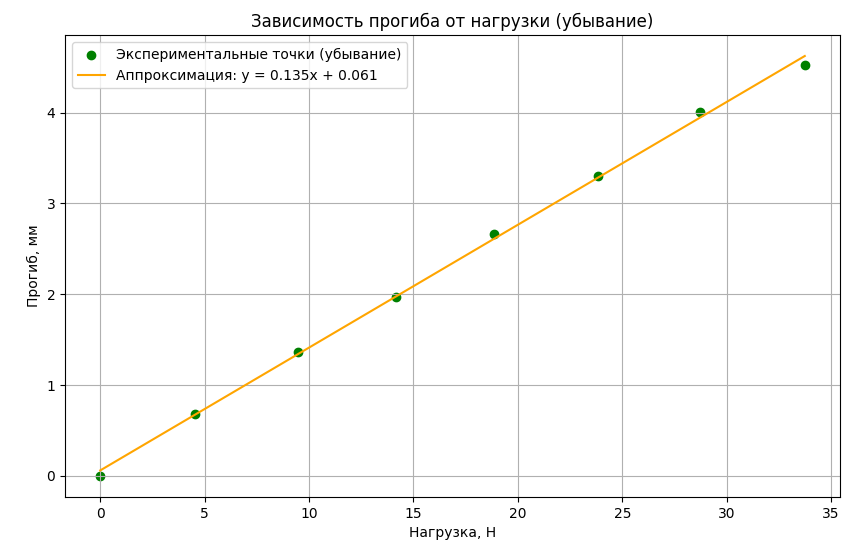
\includegraphics[width=0.8\linewidth]{G2.png}
\caption{Коэффициент угла наклона (убывание): 0.135; Модуль Юнга E = 19.17ГПа}
\label{fig:decrease}
\end{figure}


\clearpage


4.Зависимость прогиба от нагрузки (смещение 1,5\ \text{см})

\begin{table}[h]
\centering
\begin{minipage}{0.45\textwidth}
\centering
\caption{Зависимость прогиба от нагрузки (Возрастание нагрузки)}
\begin{tabular}{|c|c|}
\hline
Нагрузка, H & прогиб, мм \\
\hline
0.0 & 0.0 \\
\hline
4.585 & 0.69 \\
\hline
9.516 & 1.37 \\
\hline
14.089 & 2.0 \\
\hline
19.022 & 2.7 \\
\hline
24.035 & 3.41 \\
\hline
28.561 & 4.0 \\
\hline
33.474 & 4.7 \\
\hline
\end{tabular}
\end{minipage}
\hfill
\begin{minipage}{0.45\textwidth}
\centering
\caption{Зависимость прогиба от нагрузки (Убывание нагрузки)}
\begin{tabular}{|c|c|}
\hline
Нагрузка, H & прогиб, мм \\
\hline
33.474 & 4.7 \\
\hline
28.561 & 4.02 \\
\hline
24.035 & 3.41 \\
\hline
19.022 & 2.69 \\
\hline
14.089 & 2.04 \\
\hline
9.516 & 1.37 \\
\hline
4.585 & 0.65 \\
\hline
0.0 & 0.02 \\
\hline
\end{tabular}
\end{minipage}
\end{table}



Наблюдение: При смещении точки приложения силы от центра прогиб балки немного увеличивается.
\\[1em]

5.Измерения для перевернутой балки

\begin{table}[h]
\centering
\begin{minipage}{0.45\textwidth}
\centering
\caption{Зависимость прогиба от нагрузки (Возрастание нагрузки)}
\begin{tabular}{|c|c|}
\hline
Нагрузка, H & прогиб, мм \\
\hline
0.0 & 0.0 \\
\hline
4.526 & 0.62 \\
\hline
9.458 & 1.28 \\
\hline
14.144 & 1.89 \\
\hline
18.873 & 2.57 \\
\hline
23.817 & 3.32 \\
\hline
28.73 & 3.98 \\
\hline
33.737 & 4.48 \\
\hline
\end{tabular}
\end{minipage}
\hfill
\begin{minipage}{0.45\textwidth}
\centering
\caption{Зависимость прогиба от нагрузки (Убывание нагрузки)}
\begin{tabular}{|c|c|}
\hline
Нагрузка, H & прогиб, мм \\
\hline
33.737 & 4.49 \\
\hline
28.73 & 3.97 \\
\hline
23.817 & 3.26 \\
\hline
18.873 & 2.63 \\
\hline
14.144 & 1.94 \\
\hline
9.458 & 1.35 \\
\hline
4.526 & 0.65 \\
\hline
0.0 & 0.02 \\
\hline
\end{tabular}
\end{minipage}
\end{table}

Наблюдение: Результаты примерно такие же\\[1em]


6.Измерения для других балок

ДЛЯ МЕТАЛЛА:

\begin{table}[h]
\centering
\begin{minipage}{0.45\textwidth}
\centering
\caption{Зависимость прогиба от нагрузки (Возрастание, металл)}
\begin{tabular}{|c|c|}
\hline
Нагрузка, H & прогиб, мм \\
\hline
4.574 & 1.1 \\
\hline
9.504 & 2.22 \\
\hline
14.03 & 3.41 \\
\hline
18.962 & 4.49 \\
\hline
23.648 & 5.67 \\
\hline
28.234 & 6.75 \\
\hline
32.962 & 7.84 \\
\hline
\end{tabular}
\end{minipage}
\hfill
\begin{minipage}{0.45\textwidth}
\centering
\caption{Зависимость прогиба от нагрузки (Убывание, металл)}
\begin{tabular}{|c|c|}
\hline
Нагрузка, H & прогиб, мм \\
\hline
32.962 & 7.84 \\
\hline
28.234 & 6.7 \\
\hline
23.648 & 5.54 \\
\hline
18.962 & 4.5 \\
\hline
14.03 & 3.38 \\
\hline
9.504 & 2.23 \\
\hline
4.574 & 1.12 \\
\hline
0.0 & 0.01 \\
\hline
\end{tabular}
\end{minipage}
\end{table}

\begin{figure}[h]
\centering
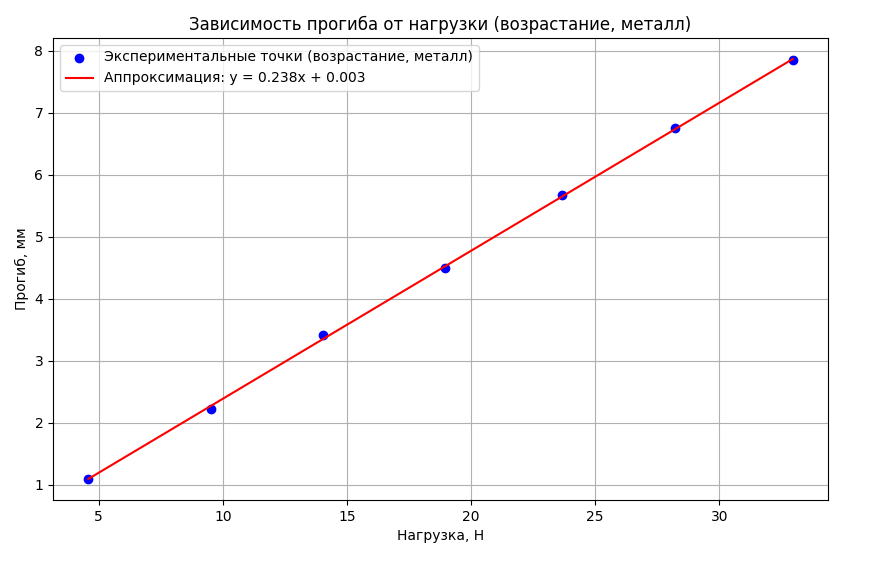
\includegraphics[width=0.8\linewidth]{G3.png}
\caption{Коэффициент угла наклона (возрастание): 0.238; Модуль Юнга E = 62.7ГПа}
\label{fig:increase}
\end{figure}


\vspace{2cm} % Добавляем вертикальное пространство между картинками

\begin{figure}[h]
\centering
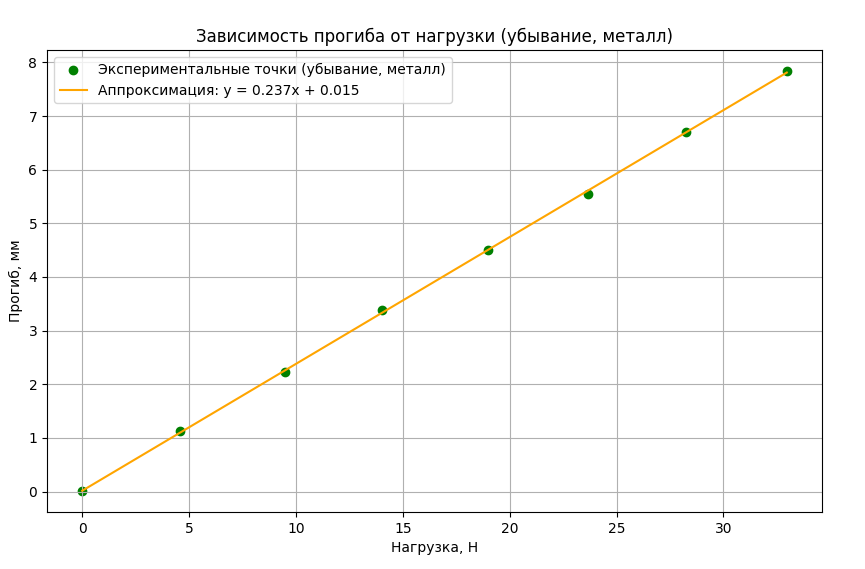
\includegraphics[width=0.8\linewidth]{G4.png}
\caption{Коэффициент угла наклона (убывание): 0.237; Модуль Юнга E = 63.4ГПа}
\label{fig:decrease}
\end{figure}


\clearpage



\begin{table}[h]
\centering
\caption{Зависимость прогиба от нагрузки (Возрастание, металл, для перевернутой балки)}
\begin{tabular}{|c|c|}
\hline
Нагрузка, H & прогиб, мм \\
\hline
4.574 & 1.08 \\
\hline
9.504 & 2.19 \\
\hline
14.03 & 3.37 \\
\hline
18.962 & 4.52 \\
\hline
23.648 & 5.63 \\
\hline
28.234 & 6.78 \\
\hline
32.962 & 7.86 \\
\hline
\end{tabular}
\end{table}

\begin{table}[h]
\centering
\caption{Зависимость прогиба от нагрузки (Убывание, металл, для перевернутой балки)}
\begin{tabular}{|c|c|}
\hline
Нагрузка, H & прогиб, мм \\
\hline
32.962 & 7.86 \\
\hline
28.234 & 6.73 \\
\hline
23.648 & 5.58 \\
\hline
18.962 & 4.47 \\
\hline
14.03 & 3.35 \\
\hline
9.504 & 2.21 \\
\hline
4.574 & 1.10 \\
\hline
0.0 & 0.03 \\
\hline
\end{tabular}
\end{table}

ДЛЯ ДРУГОЙ ДЕРЕВЯННОЙ БАЛКИ:

\begin{table}[h]
\centering
\begin{minipage}{0.45\textwidth}
\centering
\caption{Зависимость прогиба от нагрузки (Возрастание, дерево 2)}
\begin{tabular}{|c|c|}
\hline
Нагрузка, H & прогиб, мм \\
\hline
4.574 & 0.65 \\
\hline
9.099 & 1.27 \\
\hline
13.685 & 1.85 \\
\hline
18.413 & 2.45 \\
\hline
23.112 & 3.12 \\
\hline
28.032 & 3.81 \\
\hline
32.962 & 4.45 \\
\hline
\end{tabular}
\end{minipage}
\hfill
\begin{minipage}{0.45\textwidth}
\centering
\caption{Зависимость прогиба от нагрузки (Убывание, дерево 2)}
\begin{tabular}{|c|c|}
\hline
Нагрузка, H & прогиб, мм \\
\hline
32.962 & 4.45 \\
\hline
28.032 & 3.73 \\
\hline
23.1 & 3.15 \\
\hline
18.413 & 2.54 \\
\hline
13.685 & 1.91 \\
\hline
9.099 & 1.23 \\
\hline
4.574 & 0.59 \\
\hline
0.0 & 0.02 \\
\hline
\end{tabular}
\end{minipage}
\end{table}

\begin{figure}[h]
\centering
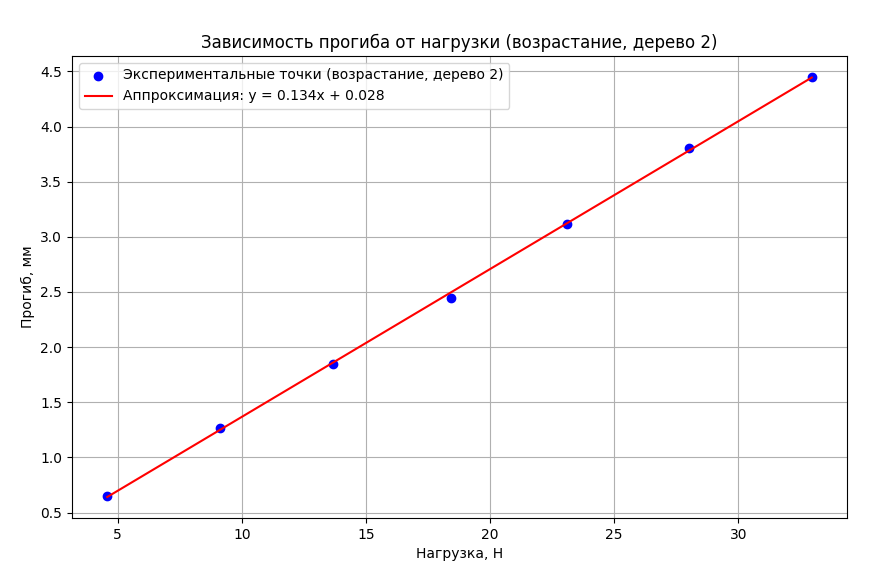
\includegraphics[width=0.8\linewidth]{G5.png}
\caption{Коэффициент угла наклона (возрастание): 0.134; Модуль Юнга E = 19.65ГПа}
\label{fig:increase}
\end{figure}


\vspace{2cm} % Добавляем вертикальное пространство между картинками

\begin{figure}[h]
\centering
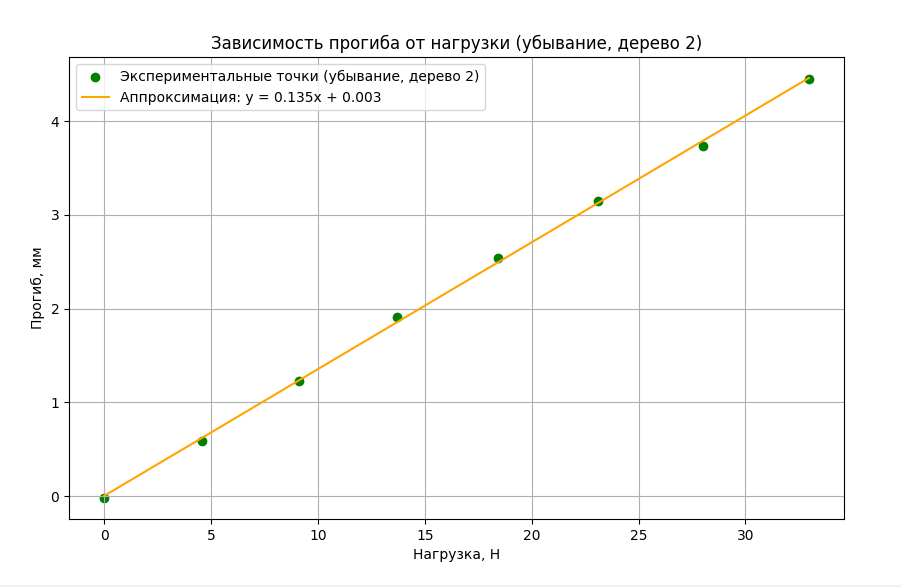
\includegraphics[width=0.8\linewidth]{G6.png}
\caption{Коэффициент угла наклона (убывание): 0.135; Модуль Юнга E = 19.84ГПа}
\label{fig:decrease}
\end{figure}


\clearpage




\begin{table}[h]
\centering
\caption{Зависимость прогиба от нагрузки (Возрастание, дерево 2, для перевернутой балки)}
\begin{tabular}{|c|c|}
\hline
Нагрузка, H & прогиб, мм \\
\hline
4.574 & 0.63 \\
\hline
9.099 & 1.25 \\
\hline
13.685 & 1.88 \\
\hline
18.413 & 2.48 \\
\hline
23.112 & 3.09 \\
\hline
28.032 & 3.77 \\
\hline
32.962 & 4.42 \\
\hline
\end{tabular}
\end{table}

\begin{table}[h]
\centering
\caption{Зависимость прогиба от нагрузки (Убывание, дерево 2, для перевернутой балки)}
\begin{tabular}{|c|c|}
\hline
Нагрузка, H & прогиб, мм \\
\hline
32.962 & 4.42 \\
\hline
28.032 & 3.75 \\
\hline
23.1 & 3.12 \\
\hline
18.413 & 2.51 \\
\hline
13.685 & 1.87 \\
\hline
9.099 & 1.21 \\
\hline
4.574 & 0.61 \\
\hline
0.0 & -0.01 \\
\hline
\end{tabular}
\end{table}

8.Погрешности оборудования

    \begin{table}[h]
        \centering
        \caption{Оборудование}
        \begin{tabular}{|c|c|}
        \hline
        Прибор         & Точность \\ \hline
        Штангенциркуль & $\pm 0.05$ мм \\ \hline
        Индикатор      & $\pm 0.01$ мм \\ \hline
        Рулетка        & $\pm 5$ мм \\ \hline
        Линейка        & $\pm 0.5$ мм \\ \hline
        Прибор Лермантова & $\pm 1$ мм \\ \hline
        \end{tabular}
    \end{table}


\section{Вывод}
Проведя ряд измерений, мы экспериментально получили зависимость между напряжением и деформацией. Учитывая погрешность измерений, полученные данные схожи с табличными.







\end{document}